% !TEX root = ../metrics_hse_exams.tex

\subsection{Demo test 1}

\begin{enumerate}
    \item We have a classical linear model 
\[
    Y_i = \beta_1 + \beta_2 X_i + u_i,
\]
where $\beta_1$ and $\beta_2$ are fixed parameters, $u_i$ is a disturbance term that is independently and identically distributed with expected value 0 and population variance $\sigma_u^2$ and $i \in \{1, \ldots, n\}$ is the observation index. 
The OLS estimation helps us to obtain the following coefficient $\beta_2$ estimator: 
\[
    \hat\beta_2 = \frac{\sum {X_iY_i}/n - \bar X \bar Y}
    {\sum {X_i^2}/n - (\bar X)^2} = 
    \frac{n \sum_{i=1}^n X_i Y_i - \sum_{i=1}^n X_i \sum_{i=1}^n Y_i}
    {n \sum_{i=1}^n X_i^2 - (\sum_{i=1}^n X_i)^2}.
\]

However, some algebraic transformations allow to show that 
\[
    \hat\beta_2 = \frac{\sum_{i=1}^n (X_i - \bar X)(Y_i - \bar Y)}
    {\sum_{i=1}^n (X_i - \bar X)^2}.
\]

Prove this is true. 

{\itshape Hint: you can try to solve backwards (going from what you are given to prove to the OLS estimator)}


\item 
A variable $Y_i$ is generated as: 
\[
    Y_i = \beta_1 + u_i,
\]
where $\beta_1$ is a fixed parameter, $u_i$ is a disturbance term that is independently and identically distributed with expected value 0 and population variance $\sigma_u^2$ and $i \in \{1, \ldots, n\}$ is the observation index. 
The least squares estimator of $\beta_1$ is $\bar Y$, the sample mean of $Y$. 
However, a researcher believes that $Y$ is a linear function of another variable $X$ and uses ordinary least squares to fit the relationship:
\[
    \hat Y_i = \hat \beta_1 + \hat \beta_2 X_i,
\]
calculating $\hat \beta_1$ as $\hat Y - \hat \beta_2 \bar X$, where $\bar X$ is the sample mean of $X$. 
Regressor $X$ may be assumed to be a nonstochastic variable. 
Determine whether the researcher’s estimator $\hat \beta_1$ is biased or unbiased, and if biased, determine the direction of the bias.


\item The output below gives the result of regressing $FDHO$, annual household expenditure on food consumed at home, on $EXP$, total annual household expenditure, both measured in dollars, using the Consumer Expenditure Survey data set. 

% \includegraphics[scale=0.44]{Stata-sample.png}

Unfortunately, some things are missing. Looking at this output, do the following tasks:

\begin{enumerate}
    \item 
    Give an interpretation of the coefficients estimations.
    
    \item
    Find the number of observations.
    
    \item
    Find the values of TSS, ESS and RSS.
    
    \item
    Explain in your own words what TSS, ESS and RSS are or provide formulas for them.
\end{enumerate}


\item We have a classical linear model 
\[
    Y_i = \beta_1 + \beta_2 X_i + u_i,
\]
where $\beta_1$ and $\beta_2$ are fixed parameters, $u_i$ is a disturbance term that is independently and identically distributed with expected value 0 and population variance $\sigma_u^2$ 
and $i \in \{1, \ldots, n\}$ is the observation index.

Derive the OLS  $\hat \beta_1$ and $\hat \beta_2$ estimators. 
Answers without a solution will not be accepted. You need to provide a full solution.
\end{enumerate}



\subsection{Test 1}

You have 40 minutes to complete the test. Please explain each step of your derivations and state all the assumptions employed. 
Note that different problems can give you different points. Maximum for the test is 10 points.  

\begin{enumerate}
    \item Some practitioners of econometrics consider regressions with transformed variables. 
    For example, if the original model specification is
\[
    Y_i = \beta_1 + \beta_2 X_i + u_i,
\]
the revised specification is
\[
    Y_i^* = \beta_1^* + \beta_2^* X_i^* + v_i,
\]
where
\[
    Y_i^* = \frac{Y_i - a}{c} \text{ and } X_i^* = \frac{X_i - b}{d}.
\]

Knowing that $a, b, c, d$ are some constants and $ c \ne 0, d \ne 0$, express the OLS estimators $\hat\beta_1^*$, $\hat\beta_2^*$ 
in terms of the OLS estimators $\hat\beta_1$, $\hat\beta_2$ [2 points].


\item A novice econometrician estimated a classical linear model 
\[
     Y_i = \beta_1 + \beta_2 X_i + u_i
\]
using 4 observations and obtained the following results:

\begin{tabular}{@{}ccccc@{}}
\toprule
 $Y_i$ & 3 & 7 & 9 & 10\\ 
 $X_i$ & 3 & XXX & XXX & 1\\ 
 $\hat Y_i$ & 4 & 8 & 7 & 11\\ 
\bottomrule
\end{tabular}

Help this econometrician find the estimates of the regression coefficients $\hat \beta_1$ and $\hat \beta_2$ [1 point] and restore the missing values in table [1 point]. 
Can you confirm that these estimations were made using the OLS method? [1 point]

\item 
The output below gives the result of regressing $WAGE$, individual monthly wage measured in thousand rubles, on $TENURE$, total years of work experience a person has.

% 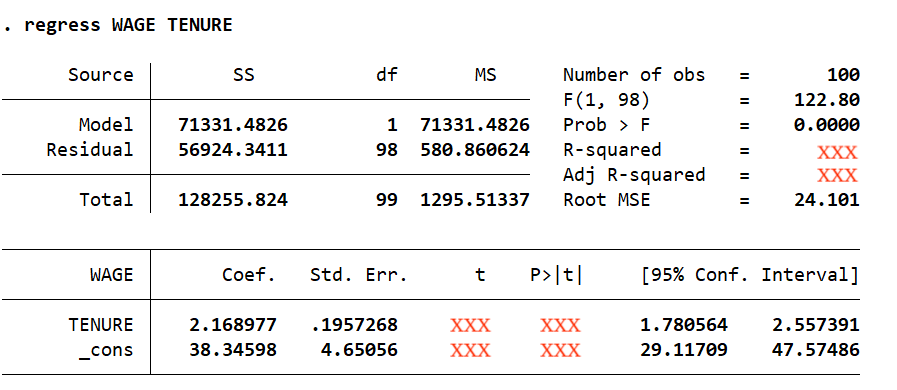
\includegraphics[scale=0.72]{Test1-model.png}

Unfortunately, some things are missing. Looking at this output, do the following tasks:

\begin{enumerate}
    \item 
    Give an interpretation of the coefficients estimations [1 point].
    
    \item
    Tell whether coefficients are statistically significant or not (if necessary, you may assume that these hypotheses are tested at a $5\%$ significance level, $t_{crit} \approx 2$) [1 point].
    
    \item
    Find the $R^2$ value [0.5 points].
    
    \item
    Explain in your own words what the $R^2$ value shows [0.5 points].
    
\end{enumerate}

\item We have a linear model 
\[
    Y_i = \beta X_i + u_i,
\]
where $\beta$ is a fixed parameter, $u_i$ is a disturbance term that is independently and identically distributed with expected value 0 and population variance $\sigma_u^2$ 
and $i \in \{1, \ldots, n\}$ is the observation index.


Derive the OLS  $\hat \beta$ estimator. 
Answers without a solution will not be accepted. You need to provide a full solution [2 points].

\end{enumerate}


\subsection{Test 2}


\subsection{Test 3}


\subsection{Test 4}
